\begin{appendices}

%Some Table of Contents entry formatting
\addtocontents{toc}{\protect\renewcommand{\protect\cftchappresnum}{\appendixname\space}}
\addtocontents{toc}{\protect\renewcommand{\protect\cftchapnumwidth}{6em}}

%Begin individual appendices, separated as chapters

\chapter{Supporting Information for chapter 3}

In this appendix, several additional experimental results are shown to characterize the formation and dynamics of travelling waves in Chapter 4. The breaking frequency and maximum wavelength are depend on the number of actuators. We also perform additional simulations of a more detailed model to assess the importance  of  amplitude  dynamics.  These simulations  reveal  that  the  approximate  model  based  on  weakly-coupled  phase  oscillators performs well for the experimental conditions.

%%%%%%%%%%%%%%%%%%%%%%%%%%%%%%%%%%%%
\begin{figure}[p]
    \centering
    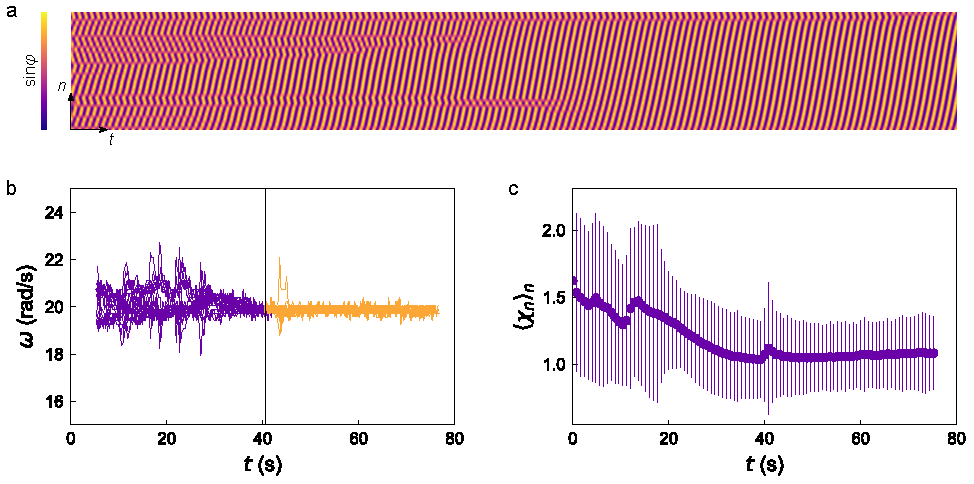
\includegraphics{figures/A2_SI1-v3.pdf}
    \caption{\textbf{Evolution of traveling waves.} (a) Full length space-time plot showing the development of traveling wave synchronization (see Figure 1d and Supplementary Movie 1). (b) Instantaneous oscillation frequency of each oscillator as a function of time during the development of synchronization. The onset of the fully synchronized state is denoted by the change in color from purple to yellow. (c) Average phase difference as a function of time during the development of synchronization. Error bars represent standard deviations in the phase difference. Data were collected for $N=23$, $a=1$ mm, $W=3$ mm, $L=25$ mm, and $V=19$ kV.}
    \label{fig:SI1}
\end{figure}


%%%%%%%%%%%%%%%%%%%%%%%%%%%%%%%%%%%%
\begin{figure}[p]
    \centering
    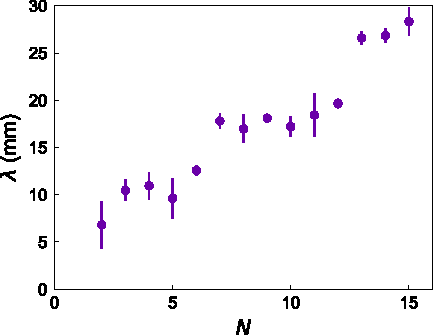
\includegraphics{figures/A2_SI2.pdf}
    \caption{\textbf{Dependence of wavelength on the number of oscillators.} Wavelength $\lambda$ (defined in the main text) as a function of the number of oscillators $N<N^*=15$. Error bars denote the standard deviation obtained over 50 cycles.  Data  were collected with $a=1$ mm, $L=25$ mm, $W=3$ mm, and $V=18$ kV.}
    \label{fig:SI2}
\end{figure}
%%%%%%%%%%%%%%%%%%%%%%%%%%%%%%%%%%%%

%%%%%%%%%%%%%%%%%%%%%%%%%%%%%%%%%%%%
\begin{figure}[p]
    \centering
    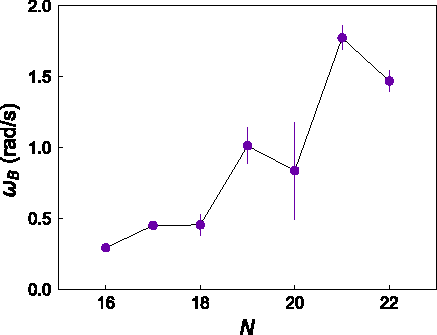
\includegraphics{figures/A2_SI3.pdf}
    \caption{\textbf{Dependence of breaking frequency on  oscillator number $N>N^*$.} Breaking frequency frequency $\omega_B$ as a function of the oscillator number $N>N^*=15$. Error bars denote standard deviations obtained over at least five breaking events. Data  were collected with $a=1$ mm, $L=25$ mm, $W=3$ mm, and $V=18$ kV.}
    \label{fig:SI3}
\end{figure}
%%%%%%%%%%%%%%%%%%%%%%%%%%%%%%%%%%%%


%%%%%%%%%%%%%%%%%%%%%%%%%%%%%%%%%%%%
\begin{figure}[p] 
    \centering
    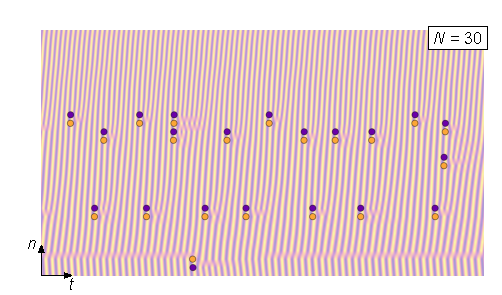
\includegraphics{figures/A2_SI4.pdf}
    \caption{\textbf{Space-time plot for $N\gg N^*$.} Space-time plot for  $N\gg N^*$ showing wave breaking at different locations and irregular time intervals. Wave breaks are characterized by edge dislocations highlighted by the markers, which show points in the space-time lattice with five-fold (purple) and seven-fold (yellow) coordination. Data were collected with $a=1$ mm, $L=25$ mm, $W=3$ mm, and $V=18$ kV. See also Supplementary Movie 5.}
    \label{fig:SI4}
\end{figure}
%%%%%%%%%%%%%%%%%%%%%%%%%%%%%%%%%%%%

%%%%%%%%%%%%%%%%%%%%%%%%%%%%%%%%%%%%
\begin{figure}[p]
    \centering
    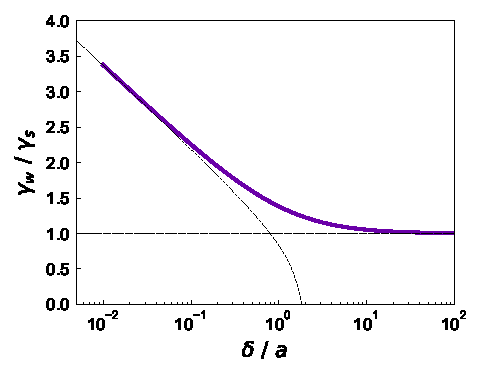
\includegraphics{figures/A2_drafCoefficient.pdf}
    \caption{\textbf{Friction coefficient for a sphere above a plane wall.} Friction coefficient $\gamma_w$ for a torque-free sphere of radius $a$ moving through a viscous fluid parallel a plane wall as a function of the surface separation $\delta$.  The friction coefficient is scaled by the Stokes drag, $\gamma_s=6\pi \eta a$, for a sphere in an unbounded fluid.  The solid curve shows the exact solution\autocite{ONeill1964a,Dean1963}; the dashed curves show the limiting behaviors for small and large surface separations.  At small separations ($\delta\ll a)$, the friction coefficient is well approximated by asymptotic expressions due to Goldman, Cox, and Brenner\autocite{Goldman1967a}.  A surface separation of $\delta = (6.4\times10^{-3})a=6.4~\mu$m would enhance the drag by the experimentally observed factor of 3.6.}
    \label{fig:SI6}
\end{figure}
%%%%%%%%%%%%%%%%%%%%%%%%%%%%%%%%%%%%


%%%%%%%%%%%%%%%%%%%%%%%%%%%%%%%%%%%%
\begin{figure}[p]
    \centering
    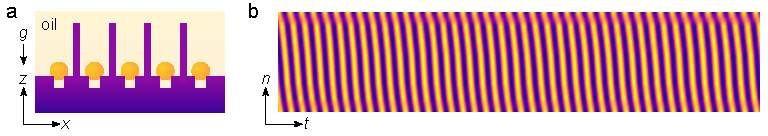
\includegraphics{figures/A2_SI5-v2.pdf}
    \caption{\textbf{Control experiments on the role of hydrodynamic interactions.} (a) Experiments were performed in which particles were separated by solid walls to eliminate hydrodynamic interactions between neighboring particles. (b) Space-time plot showing traveling wave synchronization in the absence of hydrodynamic interactions. Data were collected with  $N=8$, $a=1$ mm, $W=4$ mm, $L=25$ mm, and $V=19$ kV.}
    \label{fig:SI6}
\end{figure}
%%%%%%%%%%%%%%%%%%%%%%%%%%%%%%%%%%%%

%%%%%%%%%%%%%%%%%%%%%%%%%%%%%%%%%%%%
%%%%%%%%%%%%%%%%%%%%%%%%%%%%%%%%%%%%
\subsection{Supplementary Note 1: Amplitude dynamics}

In the main text, we model the particles as weakly-coupled phase oscillators and neglect the amplitude dynamics.  Here, we validate that approximation using numerical solutions of the corresponding ``exact'' model that includes amplitude dynamics.  In particular, we consider the dynamics of $N$ oscillators moving between two nearly parallel electrodes subject to a constant voltage $V$.  The electrode separation $L_i$ at the location of oscillator $i$ is assumed to vary linearly as $L_i=L_o - \Delta L[i + \tfrac{1}{2}(N+1)]$, where $L_o$ is the average separation and $\Delta L$ is the difference in the separation between neighboring oscillators.  The latter is related to the small angle $\theta$ between the electrodes as  $\Delta L / W =  \tan\theta \ll1$.  The external electric field acting on oscillator $i$ is approximated as $E_i=V/L_i$.

The position $h_i$ of oscillator $i$ is governed by the overdamped dynamics,
\begin{equation}
    \gamma \frac{d h_i}{d t} = q_i (E_i + E'_i),
\end{equation}
where $E'_i$ denotes the disturbance field due to neighboring particles.  The charge on oscillator $i$ changes instantaneously upon contact with the electrodes at $h_i=0$ and $h_i=L_i$. The resulting charge is
\begin{equation}
    q_i = \pm \frac{2}{3}\pi^3 \varepsilon a^2 (E_i + E'_i),
\end{equation}
where the positive sign applies at $h_i=0$ and the negative sign at $h_i=L_i$.  Again, the electric field acting on particle $i$ contains contributions from the applied field $E_i$ and from the disturbance field $E'_i$ due to neighboring particles.  In particular, the disturbance field acting on oscillator $i$ due to neighboring particles $j$ is approximated as
\begin{equation}
    E'_i = \sum_j -\frac{q_j}{L^2 \varepsilon} \sum_{m=1}^{\infty} m \sin\left(\frac{m\pi h_j}{L_j}\right) \cos\left(\frac{m\pi h_i }{L_i}\right) K_0\left(\frac{m \pi W}{L_o}\right),
\end{equation}
where the first sum is over nearest neighbors ($j=i-1$ and $i+1$) separated by a distance $W$.

It is convenient to non-dimensionalize this model by scaling lengths by $L_o$, fields by $E_o=V/L_o$, charges by $q_o=\tfrac{2}{3}\pi^3 \varepsilon a^2 E_o$, and time by $\gamma L_o/q_o E_o$.  The resulting dynamics are governed by four dimensionless parameters: (1) the number of oscillators $N$, (2) the oscillator spacing $W/L_o$, (3) electrode angle $\theta$, and (4) the coupling strength $a/W$.  We focus our analysis on the experimental conditions of Figure 2b, in which $N=15$, $W/L_o=0.12$, $\theta=1^{\circ}$, and $a/W=0.33$. The particle dynamics are integrated numerically using Mathematica's event handling feature to update the particle charges at each contact with an electrode.  At long times, the oscillators approach a steady periodic solution as illustrated in Figure \ref{fig:amplitude}.  Averaging the phase difference over one oscillation period, the results of this ``exact'' model are very well approximated by the simpler model based on weakly-coupled phase oscillators.  We note that the amplitude dynamics become more significant as the number of particles is increased from $N=10$ to $N=15$ towards the critical number of $N^*=16$.

\begin{figure}
    \centering
    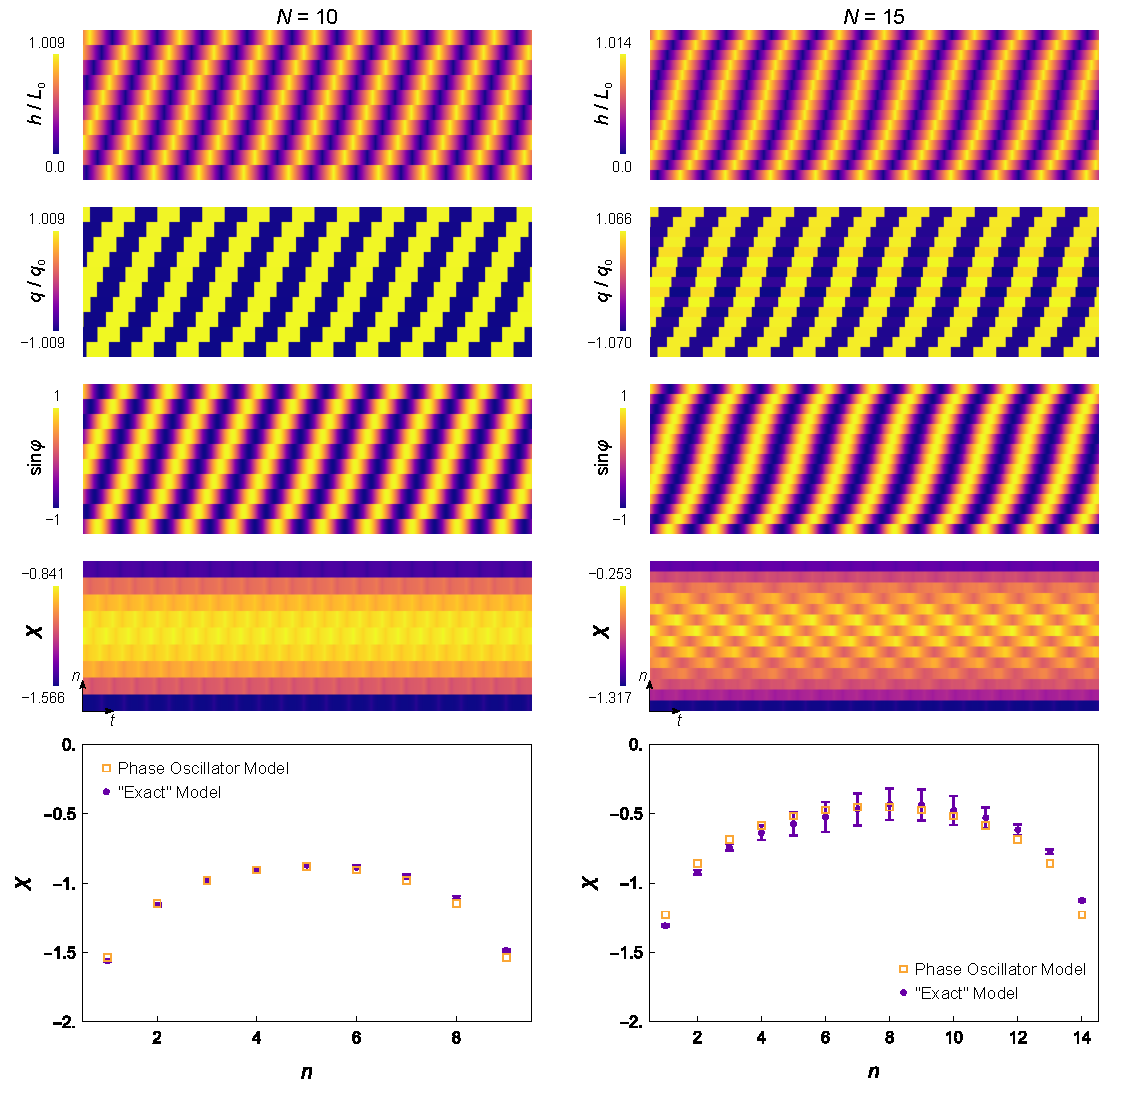
\includegraphics[width=\textwidth]{figures/A2_amplitudeDynamics.pdf}
    \caption{Numerical solution of the ``exact'' model for $N=10$ (left) and $N=15$ (right) oscillators.  The parameters are the same as those in Figure 3 of the main text: $W/L=0.12$, $a/W=0.33$, and $\theta=1^{\circ}$.  From top to bottom, the space-time plots show the particle position $h$ (scaled by the average electrode separation $L_o$), the particle charge $q$ (scaled by the Maxwell charge $q_o$), the sine of the phase $\sin\varphi$, and the phase difference $\chi$.  The plot shows the time-averaged phase difference $\chi$ as a function of the oscillator number $n$.}
    \label{fig:amplitude}
\end{figure}

\clearpage
\subsection{Supplementary Note 2: Stationary solution}

The stationary solution $f(\chi_n)=\tfrac{1}{2}\Delta n(n-N)$ is obtained by solving the following set of linear recurrence equations derived in the Methods,
\begin{align}
    \Delta &= -2 f_1 + f_2 , \label{eq:bc1}
    \\
    \Delta &= f_{n-1} - 2 f_n + f_{n+1} \quad \text{for } n=2,\dots,N-2, \label{eq:mid}
    \\
    \Delta &= f_{N-2} - 2 f_{N-1}, \label{eq:bc2}
\end{align}
where $f_n=f(\chi_n)$.  Equation (\ref{eq:mid}) has the following general solution
\begin{equation}
    f_n = C_1 + C_2 n + \frac{1}{2}\Delta n(n-1).
\end{equation}
The constants $C_1$ and $C_2$ are determined by substituting this result into the boundary conditions (\ref{eq:bc1}) and (\ref{eq:bc2}).  As the equations are linear, the resulting solution for $f_n$ is unique. However, when $|f_n| > f_{\max}$, there exists no value of the phase difference $\chi_n$ that satisfies the equation $f(\chi_n)=f_n$.  Alternatively, when $|f_n|<f_{\max}$, there exists two possible solutions for the phase difference---one with $f'(\chi_n)>0$ and another with $f'(\chi_n)<0$ as can be seen graphically in Figure 3b of the main text.

%%%%%%%%%%%%%%%%%%%%%%%%%%%%%%%%%%%%
\subsection{Supplementary Note 3: Stability of the stationary solution}

As noted above, there are two possible solutions for each of the $N-1$ phase differences.  In both experiment and simulations, we observed only one of these possible solutions in which $f'(\chi_n)<0$ for all $n$.  Here, we confirm the stability of this solution to small perturbations using a continuum approximation, in which the phase difference $\chi_n(t)$ is replaced by a continuous function $\chi(n,t)$. In this limit, the dynamics of the phase difference can be approximated as
\begin{equation}
    \frac{\partial \chi(n,t)}{\partial t} = -\frac{\partial^2 f(\chi(n,t))}{\partial n^2}  + \Delta, \label{eq:cont}
\end{equation}
subject to boundary conditions 
\begin{equation}
    f(\chi(0,t)) = f(\chi(N,t)) = 0.
\end{equation}
Note that the discrete equations for $\chi_n(t)$ correspond to a second order finite difference approximation of these continuous equations. The characteristic error introduced by this approximation is of order $(1/N)^2$, which becomes negligible for large $N$. The stationary solution $\chi_{\s}(n,t)$ is identical to that derived above for the discrete case
\begin{equation}
    \chi_{\s}(n) = \frac{1}{2} \Delta n(n-N).
\end{equation}
For small perturbations about this solution, we can approximate the function $f(\chi(n,t))$ by a first order Taylor expansion
\begin{equation}
    f(\chi(n,t)) = f(\chi_{\s}(n)) + f'(\chi_{\s}(n))[\chi(n,t)-\chi_{\s}(n)] + \dots
\end{equation}
Substituting this approximation into equation  (\ref{eq:cont}), we obtain the following diffusion equation
\begin{equation}
    \frac{\partial g}{\partial t} = -f'(\chi_{\s}(n)) \frac{\partial^2 g}{\partial n^2}, \label{eq:perturb}
\end{equation}
for the perturbation function $g(n,t)= f'(\chi_{\s}(n))[\chi(n,t)-\chi_{\s}(n)]$. Perturbations $g(n,t)$ evolve in time with a spatially dependent diffusivity $-f'(\chi_{\s}(n))$, which must be positive to ensure the decay of the perturbations and the stability of the stationary state.  Furthermore, if we approximate this diffusivity as constant, $-f'(\chi_{\s}(n))\sim f_{\max} / \chi_{\max}$, the characteristic relaxation time for equation (\ref{eq:perturb}) can be computed as $\tau \sim \chi_{\max} N^2 / \pi^2 f_{\max}$ as stated in the Methods.




\end{appendices}